\subsection{Convolution layer} \label{subs:2dconv}
In an \acrshort{cnn}, a \textbf{convolutional layer} carries out the feature extraction process of the input image, also called the input \acrfull{fm}. It is the main operation in a \acrshort{cnn} and it the layer that gives the network its name. The first layer extracts low-level features of the input \acrshort{fm} and the deepest layers use the low-level features to build an more high level one \cite{goodfellow_deep_2016}.

An input image is characterized by 3 parameters: \textbf{$N_{ix}$} the width, \textbf{$N_{iy}$} the height, and \textbf{$N_{if}$} the depth. We can illustrate then the image as a cuboid composed of layers of pixels. An illustration is presented in figure \ref{fig:notation:ifm}.
The convolution layer correlates therefore input \acrshort{fm}s and a 4D filter, to produce output \acrshort{fm}s, which contain the high-level features. The output \acrshort{fm}s are also characterized by its width $N_{ox}$, its height $N_{oy}$ and its depth $N_{of}$. We can also see a general output \acrshort{fm}s on figure \ref{fig:notation:ofm}. As a result, the filter consists of $N_{of}$ kernels, where each kernel has size $N_{kx} \times N_{ky} \times N_{if}$, that we can see in figure \ref{fig:notation:k}).
%
\begin{figure}
    \centering
    %
    \begin{subfigure}{.32\textwidth}
    \centering
    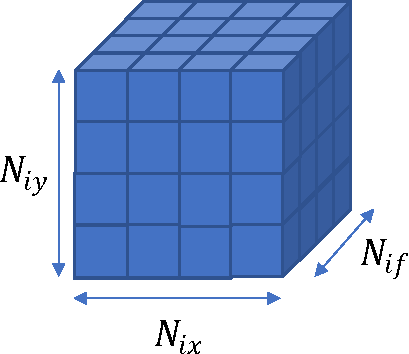
\includegraphics[width=\linewidth]{notifm.pdf}
    \caption{kernel-wise pruning}
    \label{fig:notation:ifm}
    \end{subfigure}
    %
    \begin{subfigure}{.32\textwidth}
    \centering
    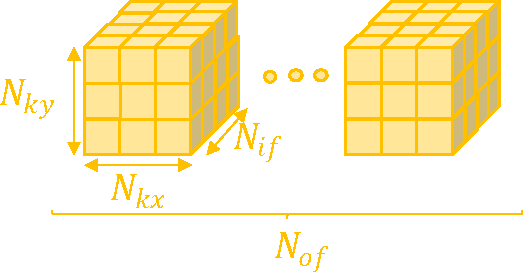
\includegraphics[width=\linewidth]{notk.pdf}
    \caption{Convolution kernel}
    \label{fig:notation:k}
    \end{subfigure}
    %
    \begin{subfigure}{.32\textwidth}
    \centering
    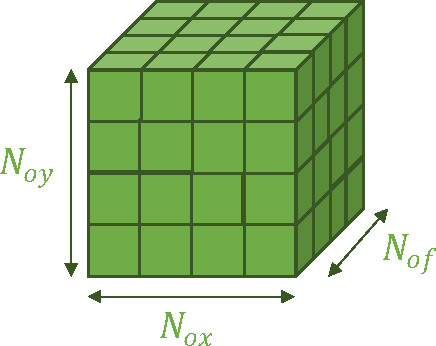
\includegraphics[width=\linewidth]{notofm.pdf}
    \caption{Output \acrshort{fm}s}
    \label{fig:notation:ofm}
    \end{subfigure}
    %
    \caption{Volumes involved in the convolution operations}
    \label{fig:notconv}
\end{figure}

Convolution is a specialized kind of linear operation. The convolution operation happens as follow. Each kernel acts as a sliding window on the input \acrshort{fm}. We extract a chunk of pixels of the same size of the kernel in the input \acrshort{fm} and perform a element-wise multiplication with the chunk of data and the kernel. We perform a sum of the computed pixels to obtain a pixel of output. Sliding this kernel on the input \acrshort{fm}s will produce a channel of the ouput \acrshort{fm}., where the output pixel at postion $(x, y)$ corresponds to the movement of the sliding window. Since one kernel produces one output \acrshort{fm}, having $N_{of}$ kernels produces then $N_{of}$ output \acrshort{fm}. An illustration of the convolution operation is in figure \ref{fig:convolution}.
%
\begin{figure}
    \centering
    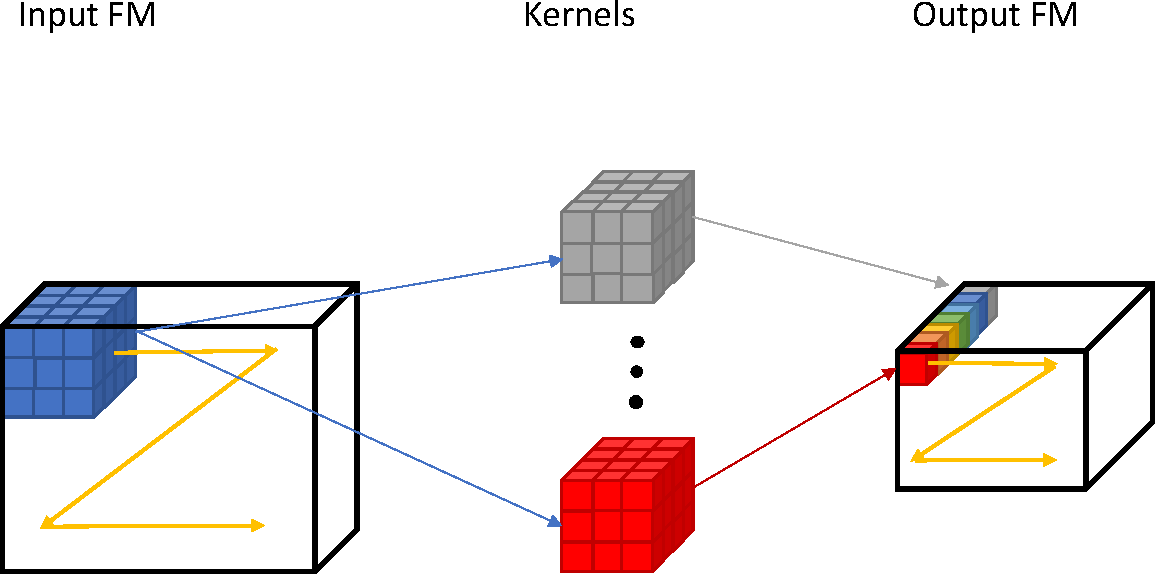
\includegraphics[width=\textwidth]{conv.pdf}
    \caption{Convolution operation}
    \label{fig:convolution}
\end{figure}

Except for $1 \times 1$ kernels, the sliding window can not cover all input pixels and then there is a spatial reduction between the input and output \acrshort{fm}s, while there is an increase in the number of channel. However, we can keep the same dimensions using \textit{padding} on the boundary (for example adding 0).

Moreover, each time the sliding window performs a convolution, it shifts in the input \acrshort{fm}. The amount by which the filter shifts is called the \textit{stride} and it is initialy set to 1. This way we can even more reduce the width and the height of the output \acrshort{fm}s. For example, if we use padding and a stride of 2, $\frac{N_{ix}}{N_{ox}} = \frac{N_{iy}}{N_{oy}} = \frac{1}{2}$ and we use 4 times less pixels.

Finally, we can express the convolution operations mathemalically as in equation \eqref{eq:conv}.
    \begin{multline}
        \forall ox \in \{ 1, ..., N_{ox} \}, oy \in \{ 1, ..., N_{oy} \}, of \in \{ 1, ..., N_{of} \} : \\
        FM_O[ox, oy, oc] = \sum^{N_{if}}_{if=1}
        \sum^{N_{kx}}_{kx=1}
        \sum^{N_{ky}}_{ky=1}
        FM_I[ox \cdot S + kx - \lfloor \frac{N_{kx}}{2} \rfloor,  oy \cdot S + ky - \lfloor \frac{N_{ky}}{2} \rfloor, if] \cdot
        W^{of}_{if}[kx, ky]
        \label{eq:conv}
    \end{multline}

If we compare the convolutional layer with the fully-connected layer, the convolutional layer allows weight sharing and then it needs less weights. For example in AlexNet \cite{krizhevsky_imagenet_2012}, 94\% of the weights are used in the fully-connected layers. But as said earlier, 90\% of the arithmetic operations are done in the convolutional layer.
